\maketitle
\setcounter{page}{1}
\newpage
\pagenumbering{arabic}
\section{Theorie}
Im folgenden werden das klassische, das einsteinsche und das Debye-Modell
zur Erläuterung der Temperaturabhängigkeit von Molwärme kristalliner Festkörper
eingeführt und diskutiert.
\subsection{Die klassische Theorie}
Klassisch gesehen verteilt sich die einem Frstkörper zugeführte Wärmeenergie gleichmäßig
auf alle Freiheitsgrade der Atome. Dies nennt man das Äquipartitionstheorem. Es gilt
\begin{equation*}
  \left< E \right> = \frac{1}{2} \, \symup{k_B} \, T
\end{equation*}
für die mittlere Energie pro Freiheitsgrad mit $T$ als Temperatur und $\symup{k_B}$ als
Boltzmannkonstante. Da diese Atome im Kristall an definierten Positionen im Gitter
sitzen, können sie entlang dreier Raumrichtungen um ihre Gleichgewichtslage schwingen.
Es folgt
\begin{equation}
  U = 3 \, N_L \, \symup{k_B} \, T = 3 \, R \, T
  \label{klassisch}
\end{equation}
für die mittlere Energie pro Atom mit $N_L$ als Loschmidtsche Zahl und $R$ als
allgemeine Gaskonstante. Die spezifische Molwärme bei konstantem Volumen ergibt
sich aus \eqref{klassisch}
\begin{equation}
  C_V = \left(\frac{\partial U}{\partial T} \right)_V = 3R \, .
  \label{eqn:1}
\end{equation}
Diese ist offensichtlich weder material- noch temperaturabhängig. Dies widerspricht
experimentellen Erfahrungen. Allerdings lässt sich der Wert $3R$ asymptotisch für
hohe Temperaturen erreichen.
\subsection{Einstein-Modell}
Die fehlende Material- und Temperaturabhängigkeit rührt daher, dass im klassischen
Ansatz die Quantelung der Schwingungsenergie außer Acht gelassen wurde. Im Einstein-Modell
schwingen alle Atome mit der Frequenz $\omega$ und können nur Schwingungsenergien
aufnehmen, die
\begin{equation}
  E = n\, \hbar \, \omega \ \ \forall \, n \in \mathbb{N}_0
  \label{eqn:2}
\end{equation}
erfüllen. Weiterhin gilt für die Wahrscheinlichkeit, mit der ein schwingendes Atom
bei einer Temperatur $T$ im thermodynamischen Gleichgewicht steht und die Energie
\eqref{eqn:2} besitzt, nach der Boltmann-Verteilung
\begin{equation}
  W(n) = \symup{exp}\left(- \frac{n \, \hbar \, \omega}{k_B \, T} \right) \, .
\end{equation}
Es gilt
\begin{equation}
  \left< U \right >_\symup{Einstein} = \frac{\sum_{n = 0}^\infty n \hbar \omega \,
  \symup{exp}\left(- \frac{n \, \hbar \, \omega}{k_B \, T} \right)}
  {\sum_{n = 0}^\infty \symup{exp}\left(- \frac{n \, \hbar \, \omega}{k_B \, T} \right)}
\end{equation}
und es folgt daraus
\begin{equation}
  \left< U \right >_\symup{Einstein} = \frac{\hbar \, \omega}
  {\symup{exp}\left(\frac{\hbar \, \omega}{k_B \, T} \right) - 1} \, .
  \label{eqn:3}
\end{equation}
Für die Molwärme ergibt sich aus \eqref{eqn:3}
\begin{equation}
  {C_V}_\symup{Einstein} = \symup{\frac{d}{dT}} 3 N_L \, \frac{\hbar \, \omega}
  {\symup{exp}\left(\frac{\hbar \, \omega}{k_B \, T} \right) - 1} =
  3R \, \frac{\hbar^2 \omega^2}{k^2 T^2} \frac{\symup{exp}\left(\hbar \omega / k_B T \right)}
  {\left[\symup{exp}\left(\hbar \omega / k_B T \right) - 1 \right]^2}
  \label{eqn:4}
\end{equation}
Für \eqref{eqn:4} gilt wie erwähnt im Grenzfall großer Temperaturen
\begin{equation}
  \lim\limits_{T \to \infty}{{C_V}_\symup{Einstein}} = 3R \, .
\end{equation}
Außerdem enthält \eqref{eqn:4} die erwartete Abnahme der Molwärme mit der Temperatur.
Allerdings weicht vor allem der Verlauf im Bereich tiefer Temperatuen stark ab vom
Verlauf der experimentellen Kurve.
\subsection{Debye-Modell}
Diese Abweichung im Bereich tiefer Temperaturen lässt sich damit erklären,
dass im Einsteinmodell von einer singulären Frequenz ausgegangen wird. Wenn man diese
ersetzt durch die spektrale Verteilung der möglichen Eigenschwingungen aller Oszillatoren
$Z(\omega)$ in einem Kristall, erhält man
\begin{equation}
  C_V = \frac{\symup d }{\symup d t} \int_0^{\omega_\symup{max}} Z(\omega) \,
  \frac{\hbar \, \omega}{\symup{exp}(\hbar \,\omega / k \, T) - 1} \symup d \omega \, .
\end{equation}
$Z(\omega)$ ist dabei recht komplizierter Natur, vor allem für z.B. anisotropes
Verhalten. Als Näherung wird angenommen, dass die Phasengeschwindigkeit unabhängig
von Frequenz und Ausbreitungsrichtung ist. $Z(\omega)$ lässt sich dann durch
einfaches Abzählen der Eigenschwingungen in einem Würfel mit Kantenlänge $L$ in
einem Frequenzintervall von $\omega$ bis $\omega + \symup d \omega$
bestimmen. Dies wird als Debye-Modell bezeichnet. Es folgt
\begin{equation}
  Z(\omega) \symup d \omega = \frac{L^3}{2\pi^2} \, \omega^2 \left(\frac{1}{{v_l}^3}
  + \frac{2}{v_{tr}^3} \right) \symup d \omega
  \label{eqn:5}
\end{equation}
mit $v_l$ und $v_{tr}$ als Phasengeschwindigkeit in longitudinaler bzw. transversaler
Richtung. Außerdem besitzt ein endlicher Kristall nur endlich viele Eigenschwingungen.
Deswegen gibt es eine Grenzfrequenz, die sogennante Debye-Frequenz, welche man aus
\begin{equation}
  \int_0^{\omega_D} Z(\omega) \symup d \omega = 3 N_L
  \label{eqn:6}
\end{equation}
erhält mit $N_L$ als Anzahl der Atome. Es folgt
\begin{equation*}
  Z(\omega) \symup d \omega = \frac{9N_L}{{\omega_D}^3} \, \omega^2 \symup d \omega
\end{equation*}
und daraus
\begin{equation}
  {C_V}_\symup{Debye} = 9 R \, \left(\frac{T}{\theta_D}\right)^3 \int_0^{\theta_D / T}
  \frac{x^4 \, \symup e^x}{(\symup e^x - 1)^2} \, \symup d x
  \label{eqn:7}
\end{equation}
mit $\theta_D$ als Debye-Temperatur, welche materialabhängig ist. Aus \eqref{eqn:7}
wird ersichtlich, dass für die Grenzfälle kleiner und großer Temperaturen
\begin{align}
  \lim \limits_{T \to \infty}{{C_V}_\symup{Debye}} &= 3R \\
  \lim \limits_{T \to 0}{{C_V}_\symup{Debye}} &\propto T^3
\end{align}
gilt. Die $T^3$-Abhängigkeit beschreibt den Grenzfall kleiner Temperaturen besser
als das Einstein-Modell, ist aber aufgrund der getroffenen Annahme immer noch eine
Näherung. Auch die Leitungselektronen tragen zur Molwärme bei, allerdings ist ihr
Beitrag erst bei tiefen Temperaturen relevant und proportional zu $T$.

\section{Durchführung}
\subsection{Versuchsaufbau}
\begin{figure}
  \centering
  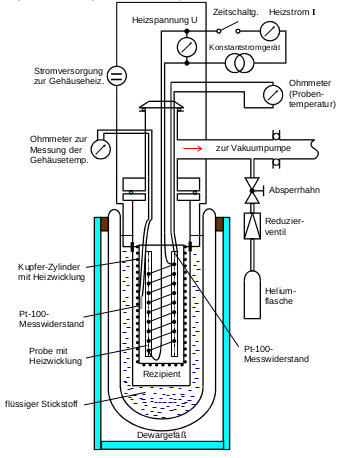
\includegraphics[scale=0.4]{aufbau.png}
  \caption{Der Versuchsaufbau im Schema.}
  \label{fig:1}
\end{figure}
In Abbildung \ref{fig:1} ist die Messapparatur zu sehen. Sie besteht aus dem Rezipienten,
in welchem sich die Probe und ein Kupferzylinder, welcher die Probe umgibt, befinden.
An der Probe und am Zylinder sind Pt-100 Messwiderständen,
deren Widerstand auf Temperaturänderungen reagiert, und Heizwicklungen angebracht.
Außen befindet sich ein Dewargefäß,
in welches der flüssige Stickstoff gefüllt wird, um die Probe und den Zylinder abzukühlen.
Die Temperaturen errechnen sich aus
\begin{equation}
  T = 0.00134 R^2 + 2.296 R - 243.02 \, ,
  \label{widerstand}
\end{equation}
wobei $R$ der Widerstand der Pt-100 Messwiderstände ist.

\subsection{Versuchsdurchführung}
Als erstes wird der Rezipient evakuiert und dann mit Helium gefüllt, um die Probe
ohne gefrierendes Wasser kühlen zu können. Sodann wird flüssiger Stickstoff in das
Dewargefäß gegeben. Sobald die Temperatur auf ca. \SI{80}{\kelvin} gesunken ist,
wird der Rezipient erneut evakuiert und die Probe in \SI{7}{\celsius}-
Schritten erwärmt. Dabei wird die benötigte Zeitdauer, die Temperaturveränderung
von Zylinder und Probe und Heizspannung und -strom aufgenommen. Es wird versucht,
den Zylinder un die Probe auf möglichst der gleichen Temperatur zu halten, damit
keine Wärmestrahlung, Konvektion oder Wärmeleitung auftreten kann. Bei ca. \SI{300}{\kelvin}
wird die Messung gestoppt.
\section{Auswertung}
\subsection{Fehlerrechnung}
Die Fehlerrechnung wird in $\textsc{Python}$\footnote{Version: 3.6.3} durchgeführt.
Mittelwerte werden durch die Funktion $\textsc{mean}$ aus dem Paket $\textsc{Numpy}$\footnote{Version: 3.6.3},
die zugehörigen Standartabweichungen durch die Funktion $\textsc{stats.sem}$ aus dem
Paket $\textsc{scipy}$\footnote{Version: 1.0.0} berechnet. Fehlerfortpflanzung wird
durch die Bibliothek $\textsc{uncertainties.unumpy}$\footnote{Version: 3.0.1} automatisiert.

\section{Diskusion}
\newpage
\nocite{*}
\printbibliography
